\documentclass[12pt]{extarticle}
%Some packages I commonly use.
\usepackage[spanish]{babel}
\usepackage{graphicx}
\usepackage{framed}
\usepackage[normalem]{ulem}
\usepackage{amsmath}
\usepackage{amsthm}
\usepackage{amssymb}
\usepackage{amsfonts}
\usepackage{enumerate}
\usepackage{alltt}
\usepackage{listings}
\usepackage[utf8]{inputenc}
\usepackage[top=1 in,bottom=1in, left=1 in, right=1 in]{geometry}

\usepackage{hyperref}
\hypersetup{
	colorlinks=true,
	linkcolor=blue,
	filecolor=magenta,      
	urlcolor=cyan,
}



\usepackage{listings}
\usepackage{color}

\definecolor{dkgreen}{rgb}{0,0.6,0}
\definecolor{gray}{rgb}{0.5,0.5,0.5}
\definecolor{mauve}{rgb}{0.58,0,0.82}

\lstset{frame=tb,
	language=C++,
	aboveskip=3mm,
	belowskip=3mm,
	showstringspaces=false,
	columns=flexible,
	basicstyle={\small\ttfamily},
	numbers=none,
	numberstyle=\tiny\color{gray},
	keywordstyle=\color{blue},
	commentstyle=\color{dkgreen}\ttfamily,
	stringstyle=\color{mauve},
	breaklines=true,
	breakatwhitespace=true,
	tabsize=3
}

\urlstyle{same}



%A bunch of definitions that make my life easier
\newcommand{\matlab}{{\sc Matlab} }
\newcommand{\cvec}[1]{{\mathbf #1}}
\newcommand{\rvec}[1]{\vec{\mathbf #1}}
\newcommand{\ihat}{\hat{\textbf{\i}}}
\newcommand{\jhat}{\hat{\textbf{\j}}}
\newcommand{\khat}{\hat{\textbf{k}}}
\newcommand{\minor}{{\rm minor}}
\newcommand{\trace}{{\rm trace}}
\newcommand{\spn}{{\rm Span}}
\newcommand{\rem}{{\rm rem}}
\newcommand{\ran}{{\rm range}}
\newcommand{\range}{{\rm range}}
\newcommand{\mdiv}{{\rm div}}
\newcommand{\proj}{{\rm proj}}
\newcommand{\R}{\mathbb{R}}
\newcommand{\N}{\mathbb{N}}
\newcommand{\Q}{\mathbb{Q}}
\newcommand{\Z}{\mathbb{Z}}
\newcommand{\<}{\langle}
\renewcommand{\>}{\rangle}
\renewcommand{\emptyset}{\varnothing}
\newcommand{\attn}[1]{\textbf{#1}}
\theoremstyle{definition}
\newtheorem{theorem}{Theorem}
\newtheorem{corollary}{Corollary}
\newtheorem*{definition}{Definition}
\newtheorem*{example}{Example}
\newtheorem*{note}{Note}
\newtheorem{exercise}{Exercise}
\newcommand{\bproof}{\bigskip {\bf Proof. }}
\newcommand{\eproof}{\hfill\qedsymbol}
\newcommand{\Disp}{\displaystyle}
\newcommand{\qe}{\hfill\(\bigtriangledown\)}

\renewcommand{\lstlistingname}{Código}% Listing-Code

\setlength{\columnseprule}{1 pt}


\title{Programación Orientada a Objetos - Apuntadores}
\author{Pedro Fernando Flores Palmeros \\ ESIME - ZACATENCO}
\date{Abril 2020}

\begin{document}

\maketitle



\section{Introducción a Apuntadores}
Una herramienta que hace que C y C++ sean muy versátiles, rápidos y muy usados, es que brindan la capacidad de poder manipular la memoria directamente mediante el uso de apuntadores.\\

Un apuntador es una variable que guarda una dirección de memoria, así como hay variables que guardan enteros, flotantes o caracteres, el puntero o apuntador guarda la dirección de memoria de una variable.\\

Suponga que en un programa se crea un variable de tipo entero \verb|int miVariable|, esta variable tendrá un tamaño de 4 bytes, en memoria se vería gráficamente algo así

\begin{figure}[thpb]
	\centering
	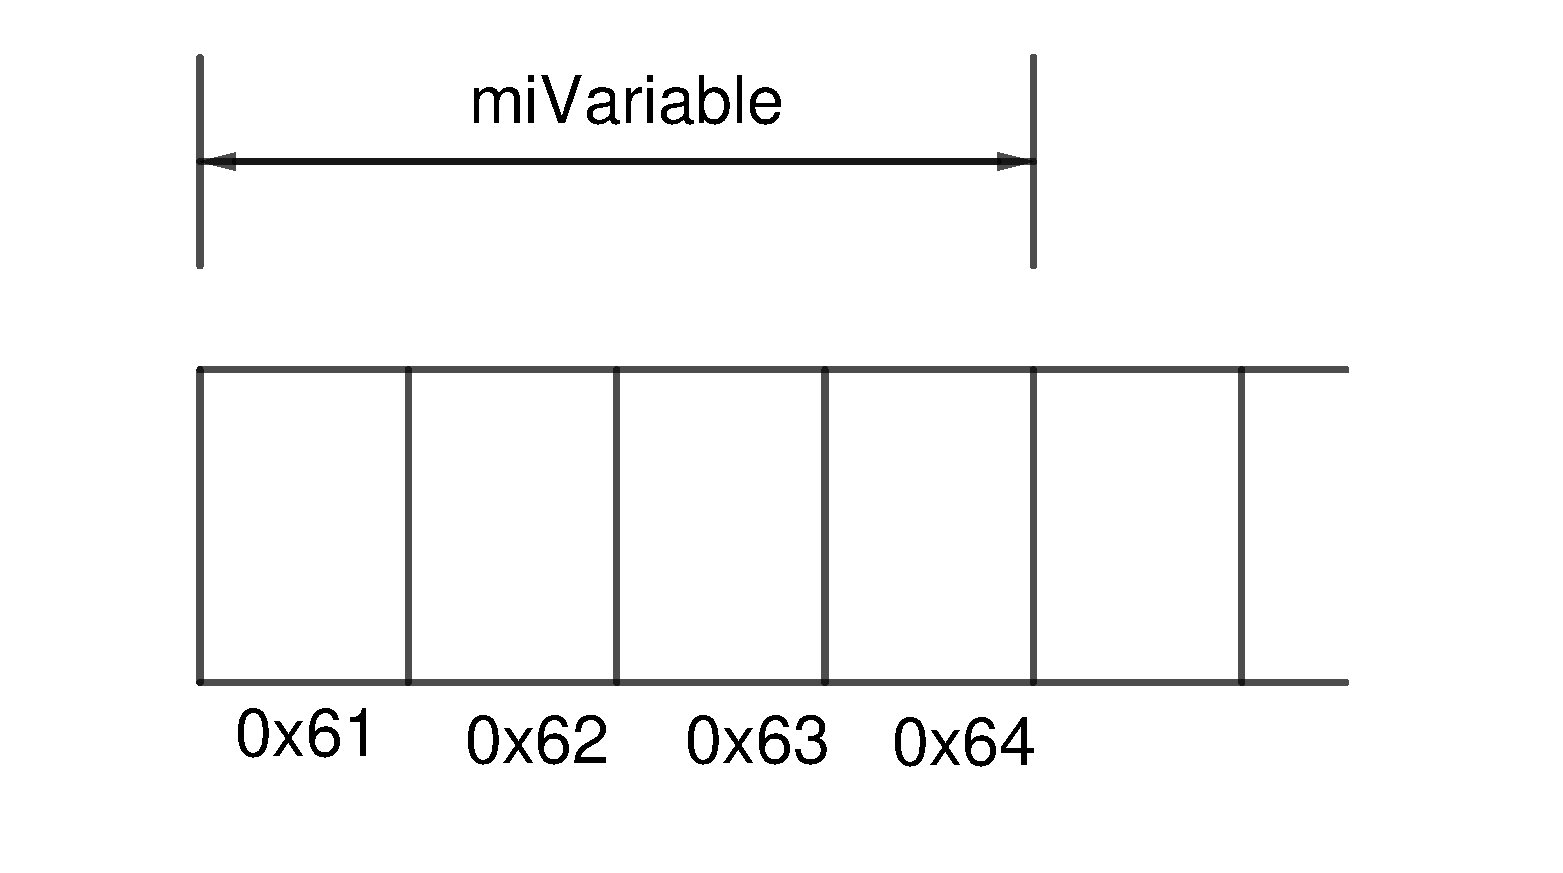
\includegraphics[scale=0.4]{Images/Memoria}      
	\caption{Representación gráfica de la memoria }
	\label{Fig::LimitCycle_01_A}
\end{figure}

Donde los números \verb|0x61, 0x62, 0x63, 0x64| son direcciones de memoria, la numeración varía entre computadoras. Por lo general lor programadores no necesitan saber la dirección de memoria tal cual, sin embargo está disponible si se utiliza el operador \verb|&|, tal como se muestra en el siguiente código


\begin{lstlisting}[caption={Obtención de la dirección de una variable},captionpos=b]
#include <iostream>

using namespace std; 

int main(){
	int miVariable = 8;
	float residuo = 69.7;
	double parametro = -6585.74;
	
	cout << "El valor de miVariable es: " << miVariable << endl;
	cout << "La direccion de miVariable es: " << &miVariable << endl; 
	cout << "-------------" << endl << endl; 
	
	cout << "El valor de residuo es: " << residuo << endl;
	cout << "La direccion de residuo es: " << &residuo << endl; 
	cout << "-------------" << endl << endl; 
	
	cout << "El valor de parametro es: " << parametro << endl;
	cout << "La direccion de parametro es: " << &parametro << endl; 
	cout << "-------------" << endl << endl; 
}
\end{lstlisting}

Y la salida en la terminal (que puede variar en la ejecución y en la computadora) sería 

\begin{lstlisting}[caption={Obtención de la dirección de una variable - Salida en terminal},captionpos=b]
El valor de miVariable es: 8
La direccion de miVariable es: 0x7ffe21733ad8
-------------

El valor de residuo es: 69.7
La direccion de residuo es: 0x7ffe21733adc
-------------

El valor de parametro es: -6585.74
La direccion de parametro es: 0x7ffe21733ae0
-------------
\end{lstlisting}

En realidad el programador no necestia conocer el valor numérico de la dirección de las variables. Lo que realmente es importante es saber que cada variable tiene una dirección y que cada variable ocupa cierta cantidad de bytes dentro del sistems. Al declarar una variable no importanto el tipo, el compilador ya sabe cuánta memoria reservar y le asigna automáticamente una dirección. \\

El apuntador debe de tener su propia memoria, sin embargo, no importa el tipo de dato al que apunte, el apuntador o puntero mantiene el tamaño.\\

\section{Definición y operadores}
Los punteros constituyen un nuevo tipo de variables, y su función principal es almacenar información. Sólo en comparación con las otras variables la naturaleza de los datos que almacena es distinta, los punteros guardan o almacenan direcciones de memoria, es dechir, hacen referencia a otra zona de memoria donde se encontrarán los verdaderos datos.\\

\subsection{Operador de dirección}

La dirección de memoria de una variable está representada por el nombre de la variable, para conocer la dirección de memoria de una variable concreta se debe de utilizar el \textbf{operador dirección} denotado por \verb|&|. Tal como se vió en primer código de este documento.\\



La sintaxis de la definición de una variable de tipo puntero es la siguiente: 
\begin{lstlisting}
tipo_dato * nombre_puntero;
\end{lstlisting}
donde \verb|tipo_dato| puede ser cualquier dato definido en C o C++, inclusive puede ser una clase o una estructura y \verb|nombre_puntero| es el nombre de la variable tipo puntero.\\

En el siguiente bloque de código se muestra un ejemplo de declaración de un puntero \verb|miPtr| y este puntero  será de naturaleza entero
\begin{lstlisting}
int * miPtr;
\end{lstlisting}
hasta ahorita sólo se ha creado el puntero, pero este puntero no está apuntando a ninguna variable, y eso puede ser peligroso. \textbf{Es una buena práctica de programación inicializar un puntero desde la declaración}, en caso de que aún no se tenga una variable que se le pueda asignar al apuntador, lo recomendable es declarar un \textbf{puntero nulo} tal como se muestra en el siguiente código

\begin{lstlisting}
int * miPtr = NULL;
\end{lstlisting}

De esta manera el apuntador se define como un puntero nulo. Sin embargo, un puntero nulo no tiene mucha utilidada, lo anterior sólo se hizo para proteger el programa. para asignar una dirección  se de extraer la dirección de una variable existente y esa dirección se puede asignar a la variable tipo puntero. Observe el siguiente ejemplo.

\begin{lstlisting}
#include <iostream>

using namespace std;

int main(){
	
	int miVar = 8;
	int * miPtr = NULL;
	miPtr = &miVar;
	
	cout << "El valor de miVar es: " << miVar << endl; 
	cout << "La direccion de miVar es: " << &miVar << endl;
	cout << "El valor de miPtr es: " << miPtr << endl; 
	
}
\end{lstlisting}

y la salida de este programa es: 

\begin{lstlisting}
El valor de miVar es: 8
La direccion de miVar es: 0x7ffe71732edc
El valor de miPtr es: 0x7ffe71732edc
\end{lstlisting}

Observe que ahora \verb|miPtr| tiene la dirección de la variable \verb|miVar|. Con lo anterior queda demostrado que el puntero es capaz de guardar la dirección de las variables. Ha sido un gran avance, sin embargo, al inicio de esta sección se mencionó que no es muy útil saber la dirección numérica del puntero. 

\begin{figure}[thpb]
	\centering
	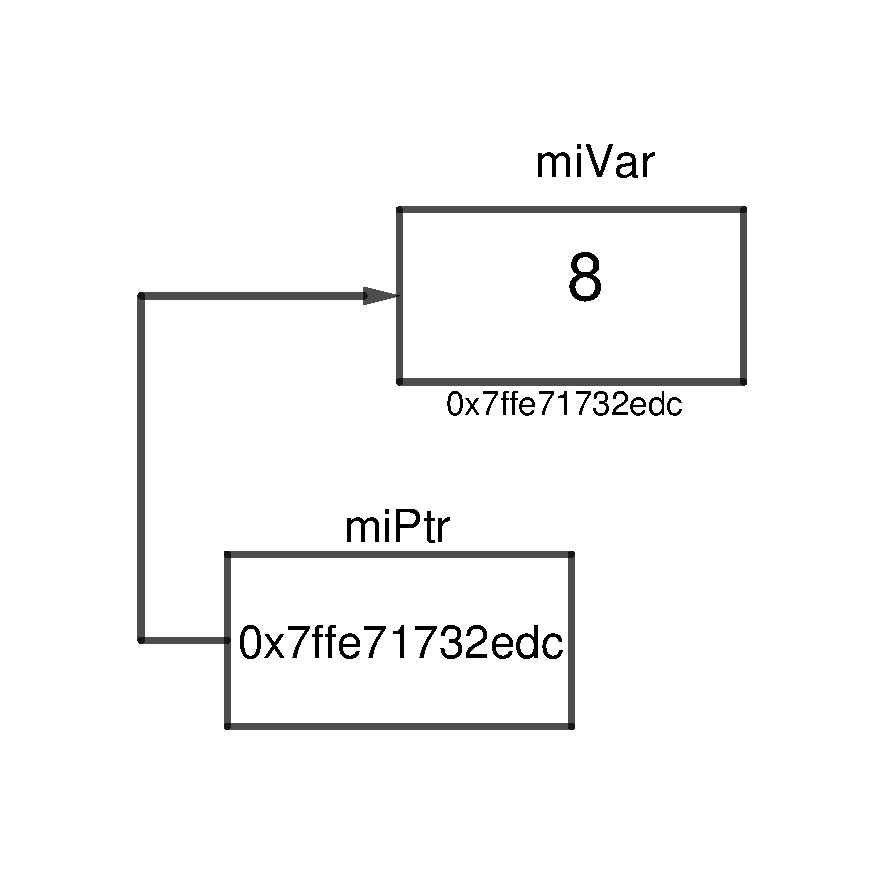
\includegraphics[scale=0.4]{Images/Prog_01}      
	\caption{Representación gráfica de la memoria }
	\label{Fig::Prog_01}
\end{figure}

En la Fig (\ref{Fig::Prog_01}) se muestra de manera gráfica el programa anterior. Observe que se han generado dos rectángulos el primero representa a la variable \verb|miVar| y tiene la dirección de memoria \verb| 0x7ffe71732edc|, observe que dentro del rectángulo de \verb|miVar| se ha puesto el número 8, que corresponde a la asignación en el momento que se ha declarado la variable. Observe que se ha puesto otro rectángulo que pertenece al puntero \verb|miPtr|, si el puntero estuviera vacío o declarado como nulo, debería de tener la palabra \verb|NULL| dentro pero en la imagen ya se muestra la dirección de la variable \verb|miVar| entonces este puntero ya ha sido asignado.


\subsection{Operador de indirección}
El \textbf{operador de indirección}  es el encargado de acceder al dato almacenado en una dirección de memoria, la cual generalmente se obtiene a paratir de una barialge de tipo puntero.\\

La sintaxis del operadro de indirección es la siguiente
\begin{lstlisting}
* Nombre_puntero
\end{lstlisting}

Este operador realiza la acción puesta al operador de dirección, permitiendo acceder a los datos localizados en una dirección de memoria. Este operador no se puede aplicar directamente a ninguna variable que no se de tipo puntero.\\

En otras palabras, para poder inicializar el puntero se le debe de mandar una dirección y se hace através del operador de dirección \verb|&| y para saber el dato al cual se está apuntando se debe de utilizar el operador indirección \verb|*|.\\

\textit{Indirección} significa acceder al valor de una variable cuyadirección está guardada en un apuntador. El puntador porporciona una manera indirecta de obtener el valor que se guarda en esa dirección.\\

Observe el siguiente boque de código.

\begin{lstlisting}
#include <iostream>

using namespace std;

int main(void){
	int Dato = 100;
	int * ptrDato = &Dato;
	
	int Valor = 0;
	
	cout << "La direccion de Dato es: " << &Dato << endl;
	cout << "El valor de Dato es: " << Dato << endl; 
	
	cout << "El valor de ptrDato es: " << ptrDato;
	cout << "El valor de la memoria a la que apunta ptrDato es: " << *ptrDato << endl;
	
	cout << "El valor de Valor es: " << Valor << endl; 
	
	Valor = *ptrDato;
	
	cout << "El nuevo valor de Valor es: " << Valor << endl; 
	
	*ptrDato = 58;
	
	cout << "El nuevo valor de Dato es: " << Dato << endl; 
}
\end{lstlisting}

En donde primero se declara la variable \verb|Dato| y se inicializa con el valor de \verb|100|, después se declara un putero tipo entero \verb|* ptrDato| y se inicializa con la dirección de \verb|Dato| debido a que tiene \verb|int *ptrDato = &Dato|, se declara e inicializa la variable \verb|Valor| y se inicializa con \verb|0|. Se imprimen los valores de la \verb|Dato| y de \verb|ptrDato|, y depués se hace \verb|Valor=*ptrDato|, esta instrucción sería similar a \verb|Valor = Dato|, \verb|*ptrDato| extrae el valor de \verb|Dato| no la dirección, a este hecho se le conoce como \textit{desreferencia o indirección}. Después se hace \verb|*ptrDato = 58| pero como \verb|ptrDato| apunta a \verb|Dato| en realidad se está modificando el valor de \verb|Dato| de manera indirecta a través del puntero. \\

El operador de indirección \verb|*| se utiliza de dos maneras distintas con lso aputnadores: declaración y desreferencia. Cuando se declara un apuntador el asterisco indica que es unaputador, no una variable normal.\\

Cuando el puntador es desreferenciado, el operador de indirección indica que se debe de acceder al valor que se encuentra en la dirección de meoria guardada en el apuntador, y no a la dirección en sí.\\

\section{¿Por qué utilizar apundaores?}

La memoria de la computadora básicamente se puede dividir en partes (o por lo menos para el análisis que se muestra en esta sección), la primera es la RAM, que es más rápida, cara y muy limitada en los equipos de cómputo. y está la ROM que generalmente es abundante y muy económica, en un equipo de cómputo la ROM sería el disco duro (para fines prácticos), los programas que se han desarrollado se compilan y cuando se ejecutan se reserva una candiad determinada de memoria en RAM, en esa sección están las variables, funciones, etc, sin embargo, la memoria RAM es limitada. Suponga a hora que quiere hacer varios objetos de alguna clase, si estos objetos son muy grandes comenzarán a consumir más y más memoria RAM, haciendo que el programa y el equipo en general se más lento. Una de las formas de eficientar todo esto es que el programa principal esté en la memoria del programa (RAM) y los objetos o estructuras que son más grandes estén en la memoria ROM y para poder acceder de la RAM a la ROM se utilizan los apuntadores, ya que la ROM es una memoria seccionada y muy organizada.\\

La memoria asignada a los programas a través del compilador se asigna,reserva y libera de forma automática, sin embargo, la memoria en la ROM debe de ser administrada de manera manual por el programador.\\

Por lo general, los apuntadores se utilizan para tres cosas:
\begin{itemize}
	\item Manejar datos en el \verb|heap| (heap en español es montículo y hace referencia a la memoria ROM).
	\item Tener acceso a los datos miembro y a las funciones de las clases. 
	\item Pasar variables por referencia a las funciones.
\end{itemize}

\section{new}
Supongamos que se quiere hacer un apuntador en C++, que sería  con la forma que se ha explicado en las secciones anteriores. 

\begin{lstlisting}
int * miApuntador;
\end{lstlisting}

Este apuntador está a la deriva, para asignarle una dirección de memoria en el heap se debe de utilizar la palabra \verb|new| como se muestra en el siguiente bloque de código

\begin{lstlisting}
miApuntador = new int; 
\end{lstlisting}

Si se quisiera declarar e inicializar el apuador, que es lo más recomendable tendría que ser de la siguiente forma: 

\begin{lstlisting}
int * miApuntador = new int; 
\end{lstlisting}


\section{delete}
Al terminar de utilizar la memoria en el heap, es recomendable liberar el espacio utilizado, para esto, es necesario llamar  a la instrucción \verb|delete|  para liberar la memoria reservada.  

\begin{lstlisting}
delete miApuntador;
\end{lstlisting}

Si se ha reservado memoria a través de \verb|new| y esta no se libera y se termina de ejecutar el programa y la memoria nunca se liberó, entonces esa memoria quedará reservada y no habrá manera de acceder a ella, a menos que se reinicie el equipo, a este fenómeno se le conoce como \textit{fuga de memoria}.\\

Observe el siguiente bloque de código donde se alcanza a apreciar el uso de las dos nuevas palabras reservadas. 

\begin{lstlisting}
#include <iostream>

using namespace std; 

int main(){
	int miVariable = 8;
	int * apLocal = &miVariable;
	int * apHeap = new int;
	
	*apHeap = 90;
	cout << "El valor de miVariable es: " << miVariable << endl; 
	cout << "El valor al que apunto apLocal es: " << *apLocal << endl;
	cout << "El valor al que apunto apHeap es: "  << *apHeap << endl; 
	delete apHeap;
	
	
	int * apHeap_01 = new int;
	*apHeap_01 = 54;
	cout << "*apHeap_01: " <<  *apHeap_01<< endl;
	delete apHeap_01;
}
\end{lstlisting}


\section{Objetos fuera de la memoria del programa}

Así como se puede crear un apuntador a un entero o a un flotante, también se puede crear un apuntador a cualquier objeto. Como se ha mencionado con anterioridad, es recomendable que variables, estructuras y objetos estén ubicados en el Heap y no de manera local para evitar la saturación de memoria. 

Considere la clase \verb|Felino| que se muestr a continuación

\begin{lstlisting}
#include <iostream>
#include <string>

using namespace std;

class Perro{
	private:
	int Edad;
	string Nombre;
	
	public:
	Perro();
	~Perro();
};

Perro::Perro(){
	cout << "Se ha llamado al constructor" << endl;
	Edad = 1;
	Nombre = "perro";
}

Perro::~Perro(){
	cout << "Se ha llamado al destructor" << endl; 
}
\end{lstlisting}


\begin{lstlisting}
#include <iostream>
#include "perro.h"

using namespace std;

int main(){
	cout << "Se va a crear un Perro local" << endl; 
	Perro Pancho;
	
	cout << "Se va acrear un Perro en el heap" << endl; 
	Perro *Orejas = new Perro;
	
	cout << "Se borrara el Perro del heap" << endl; 
	delete Orejas;
	
	cout << "Fin del programa" << endl;
	
}
\end{lstlisting}


\begin{lstlisting}
Se va a crear un Perro local
Se ha llamado al constructor
Se va acrear un Perro en el heap
Se ha llamado al constructor
Se borrara el Perro del heap
Se ha llamado al destructor
Fin del programa
Se ha llamado al destructor
\end{lstlisting}

Observe que en la salida del programa se crea un objeto de manera local y otro en el Heap, sin embargo, se debe de liberar la memoria del perro creado en el heap, para esto se utiliza \verb|delete|, y cuando se utiliza esta instrucción se manda a llamar al destructor de la clase. Note que el destructor para el perro local no es necesario llamaro debido a que esto lo hace el programa de manera automática. 






\section{Acceso a los datos miembro de punteros a objetos}
Si se tiene un objeto, se ha mencionad en las secciones anteriores, que para poder utilizar o invocar los métodos se hace a través del operador punto (\verb|.|), esto es valido para objetos creados de forma local, Para tener acceso a los métodos de un objeto que está en el heap se tiene que desreferncial el apunto y llamar al operador punto en el objeto. Observe el siguiente ejemplo donde se muestra cómo entrar al método \verb|ladrar()| sólo que en el primer caso es de un objeto creado de manera local y el segundo es de un objeto creado en el heap.

\begin{lstlisting}
PerroLocal.ladrar();
(*PerroHeap).ladrar();
\end{lstlisting}

Los paréntesis se utilizan para asegurar que \verb|PerroHeap| sea desreferenciado antes de tener acceso a \verb|ladrar()|.\\

Esto podría parecer bastante extraño, C++ proporciona un perador de método abrebiado para el acceso indirecto: el operador de flecha \verb|->|. de tal manero que las dos líneas que se muestran a continuación son equivalentes

\begin{lstlisting}
(*PerroHeap).ladrar();
PerroHeap->ladrar();
\end{lstlisting}

A continuación se muestra un ejemplo donde se puede observar de manera completa la implementación de estos términos nuevos.\\

El archivo cabezera sería el siguiente 

\begin{lstlisting}
#include <iostream>
#include <string>

using namespace std;

class Perro{
	private:
	int Edad;
	string Nombre;
	
	public:
	Perro();
	~Perro();
	void asignarEdad(int A);
	int obtenerEdad()const;
	void asignarNombre(string N);
	string obtenerNombre()const;
	void ladrar();
	void imprimirInfo();
};

Perro::Perro(){
	cout << "Se ha llamado al constructor" << endl;
	Edad = 1;
	Nombre = "perro";
}

Perro::~Perro(){
	cout << "Se ha llamado al destructor" << endl; 
}

void Perro::asignarEdad(int A){ Edad = A; }
int Perro::obtenerEdad()const{ return Edad;}
void Perro::asignarNombre(string N){ Nombre = N;}
string Perro::obtenerNombre()const{return Nombre;}
void Perro::ladrar(){cout << "Grrrauuuu " << endl; }
void Perro::imprimirInfo(){
	cout << "El perro: " << Nombre << endl; 
	cout << "Tiene: " << Edad << " anios de edad" << endl;
}
\end{lstlisting}

\begin{lstlisting}
#include <iostream>
#include "perro.h"

using namespace std;

int main(){
	
	cout << "Se crea un perro en en el Heap" << endl; 
	Perro *PerroHeap01 = new Perro;
	
	(*PerroHeap01).asignarNombre("Orejas");
	PerroHeap01->asignarEdad(7);
	(*PerroHeap01).imprimirInfo();
	PerroHeap01->imprimirInfo();
	
	delete PerroHeap01;
	
}
\end{lstlisting}

La salida del programa es

\begin{lstlisting}
Se crea un perro en en el Heap
Se ha llamado al constructor
El perro: Orejas
Tiene: 7 anios de edad
El perro: Orejas
Tiene: 7 anios de edad
\end{lstlisting}


\section{Métodos fuera de la memoria del programa} 
Uno o más de los datos miembro de una clase pueden ser apuntadores a un objeto que se encuentre en el heap, estos se deben de inicializar en el constructor y también se deben de destruir en el destructor, tal como se muestra en el siguiente bloque de código.

\begin{lstlisting}
#include <iostream>
#include <string>

using namespace std;

class Perro{
	private:
	int * Edad;
	string * Nombre;
	
	public:
	Perro();
	~Perro();
	void asignarEdad(int A);
	int obtenerEdad()const;
	void asignarNombre(string N);
	string obtenerNombre()const;
	void ladrar();
	void imprimirInfo();
};

Perro::Perro(){
	cout << "Se ha llamado al constructor" << endl;
	Edad = new int;
	Nombre = new string;
	*Edad = 5;
	*Nombre = "Dogggi";
	
}

Perro::~Perro(){
	cout << "Se ha llamado al destructor" << endl; 
	cout << "Se eliminaran todos los objetos en el heap" << endl;
	delete Edad;
	delete Nombre;
	
}

void Perro::asignarEdad(int A){ *Edad = A; }
int Perro::obtenerEdad()const{ return *Edad;}
void Perro::asignarNombre(string N){ *Nombre = N;}
string Perro::obtenerNombre()const{return *Nombre;}
void Perro::ladrar(){cout << "Grrrauuuu " << endl; }
void Perro::imprimirInfo(){
	cout << "El perro: " << *Nombre << endl; 
	cout << "Tiene: " << *Edad << " anios de edad" << endl;
}
\end{lstlisting}





\begin{lstlisting}
#include <iostream>
#include "perro.h"

using namespace std;

int main(){
	
	cout << "Se crea un perro en en el Heap" << endl; 
	Perro *PerroHeap01 = new Perro;
	
	(*PerroHeap01).asignarNombre("Orejas");
	PerroHeap01->asignarEdad(7);
	(*PerroHeap01).imprimirInfo();
	PerroHeap01->imprimirInfo();
	
	delete PerroHeap01;
	
}
\end{lstlisting}



\section{Apuntador $this  ->$}

Toda función miembro de esta clase tiene un parámetro oculto: el apuntador \verb|this|. El apuntador \verb|this| apunta al propio objeto. Por lo tanto en cada llamada de algún método de la clase se pasa el apuntador \verb|this| de forma oculta. Y es una buena pŕactica utilizar este apuntador para hacer referencia a los atributos que pertenecen a la clase, de esta manera se evitan confusiones en caso de que pudieran existir variables repetidas.\\

Observe la siguiente clase y la aplicación del apuntador \verb|this| 

\begin{lstlisting}
#include <iostream>
#include <string>

using namespace std;

class Perro{
	private:
	int Edad;
	string Nombre;
	
	public:
	Perro();
	~Perro();
	void asignarEdad(int Edad);
	int obtenerEdad()const;
	void asignarNombre(string Nombre);
	string obtenerNombre()const;
	void ladrar();
	void imprimirInfo();
};

Perro::Perro(){
	cout << "Se ha llamado al constructor" << endl;
	this->Edad = 1;
	this->Nombre = "perro";
}

Perro::~Perro(){
	cout << "Se ha llamado al destructor" << endl; 
}

void Perro::asignarEdad(int Edad){ this->Edad = Edad; }
int Perro::obtenerEdad()const{ return this->Edad;}
void Perro::asignarNombre(string Nombre){ this->Nombre = Nombre;}
string Perro::obtenerNombre()const{return this->Nombre;}
void Perro::ladrar(){cout << "Grrrauuuu " << endl; }
void Perro::imprimirInfo(){
	cout << "El perro: " << this->Nombre << endl; 
	cout << "Tiene: " << this->Edad << " anios de edad" << endl;
}
\end{lstlisting}




\section{Apuntadores const}



\begin{lstlisting}
#include <iostream>

using namespace std;

int main(){
	int A = 7;
	int B = 155;
	int C = -97;
	
	int *ptrA = &A;
	
	cout << "ptrA está apuntando a A y el valor de *ptrA es: " << *ptrA << endl; 
	*ptrA = -978;
	cout << "Se ha cambiando el valor de *ptrA, se cambia el valor de A: " << *ptrA << endl;
	
	ptrA = &B;
	
	cout << "ptrA está apuntando a B y el valor de *ptrA es: " << *ptrA << endl; 
	
	
	const int * ptrB = &B;
	
	cout << "ptrB está apuntando a B y el valor de *ptrB es: " << *ptrB << endl;
	
	
	// Si se descomenta maracara error
	//*ptrB = -1;
	//cout << "se ha cambiado *ptrB, ahora B vale: " << *ptrB << endl;  
	
	int * const ptrC = &C;
	
	cout << "ptrC apunta a C" << endl; 
	cout << "Se quiere cambiar el apuntador: " << endl;
	
	ptrC = &A;
}
\end{lstlisting}

\section {Apuntadores const y funciones miembro const} 

\end{document}
